\documentclass[11pt,a4paper]{article}

\usepackage[utf8]{inputenc}
\usepackage[T1]{fontenc}
\usepackage[margin=2.2cm]{geometry}
\usepackage{amsmath}
\usepackage{graphicx}
\usepackage{booktabs}
\usepackage{array}
\usepackage{caption}
\usepackage{xcolor}
\usepackage{hyperref}
\hypersetup{colorlinks=true,linkcolor=blue!50!black,urlcolor=blue!50!black,citecolor=blue!50!black}
\captionsetup{font=small,labelfont=bf}

\newcommand{\view}[3]{\includegraphics[width=0.235\textwidth]{#1/GLM/Condition_#2/HbO/cond-#2-#3-HbO.png}}
\newcommand{\viewrow}[2]{\view{#1}{#2}{left} & \view{#1}{#2}{right} & \view{#1}{#2}{anterior} & \view{#1}{#2}{superior}}

\title{Piano playing in quiet and in pink noise:\\ a single-subject fNIRS pilot (LYDIA)}
\author{Adam Emile Aske}
\date{2026-09-07}

\begin{document}
\maketitle

\begin{abstract}
\noindent One pianist played a memorised piece in a music recording studio, alternating $\sim$40\,s play blocks with $\sim$30\,s rest, in four sessions: two in quiet (QUIET) and two with pink noise from a loudspeaker to the left of the player (NOISE). Prefrontal, premotor/SMA, sensorimotor and temporal cortex were recorded with a 16$\times$16 NIRSport2 montage (47 channels). A subject-level AR-IRLS GLM (NIRWizard 0.1.7 / cedalion) found widespread play-related HbO increases in both conditions (44--45 of 47 channels at FDR $q<0.05$). Thresholding the $t$-maps at $|t|>10$ separates the two conditions: QUIET is dominated by prefrontal, left premotor and left temporal channels, while NOISE adds a right temporal--ventral premotor cluster (T8--FT8, T8--C6, FC6--C6) that is absent in QUIET. The HbO laterality index drops from $+0.12$ (QUIET) to $+0.06$ (NOISE), i.e.\ toward bilateral. The effect is descriptive (one subject, no QUIET-vs-NOISE contrast, no channel QC applied) but is a clear candidate hypothesis for the cohort study.
\end{abstract}

\section{Methods}

\subsection{Participant, task and sessions}
A single pianist (sub-01) played a memorised piece on a real piano in a music recording studio. In the NOISE condition a loudspeaker placed to the \emph{left} of the player emitted pink noise; in QUIET the room was silent. No ECG and no MIDI were recorded. Sessions were run in the order \texttt{quiet\_1} (ses-08), \texttt{noise\_1} (ses-09), \texttt{quiet\_2} (ses-10), \texttt{noise\_2} (ses-11), all on 2026-09-07. Each session was one run of 6 play blocks (planned $40\pm8$\,s, jittered) separated by rest ($30\pm5$\,s), preceded by a 60\,s baseline; a 1\,kHz beep cued each play (1 beep) and rest (2 beeps) onset. Markers were sent over LSL (20 = play/QUIET, 21 = play/NOISE, 30 = rest). Executed play blocks lasted 32--46\,s (mean 38.4\,s, \texttt{data/blocks.csv}). Because Aurora stores every marker with a 10\,s duration, the \texttt{.snirf} files were copied with the play markers set to 40\,s (\texttt{data/dur40/}) before analysis; the GLM therefore models a 40\,s boxcar for every play block ($n=12$ onsets per condition).

\subsection{Montage and acquisition}
The \texttt{PianoNoise} montage (Fig.~\ref{fig:montage}) uses 16 sources and 16 detectors on 10-10 sites, giving 47 channels of 30--42\,mm separation (mean 35.4\,mm) and no short-separation channels. Coverage: frontal pole/VLPFC (Fpz, AF7, AF8 $\rightarrow$ Fp1, Fp2, AFz), DLPFC (AF3, AF4, Fz, F3, F4 $\rightarrow$ F5, F1, F2, F6), premotor/SMA (FC5, FC1, FC2, FC6 $\rightarrow$ FC3, FCz, FC4), sensorimotor (C3, C4 $\rightarrow$ C5, C6) and temporal (T7, T8 $\rightarrow$ FT7, TP7, FT8, TP8). The hemispheres are joined only across the prefrontal midline (AFz, Fz, FCz); the motor and temporal strips are separate left/right chains. Data were acquired with a NIRSport2 (Aurora 2025.2) at 760/850\,nm and 12.2\,Hz.

\begin{figure}[htbp]
\centering
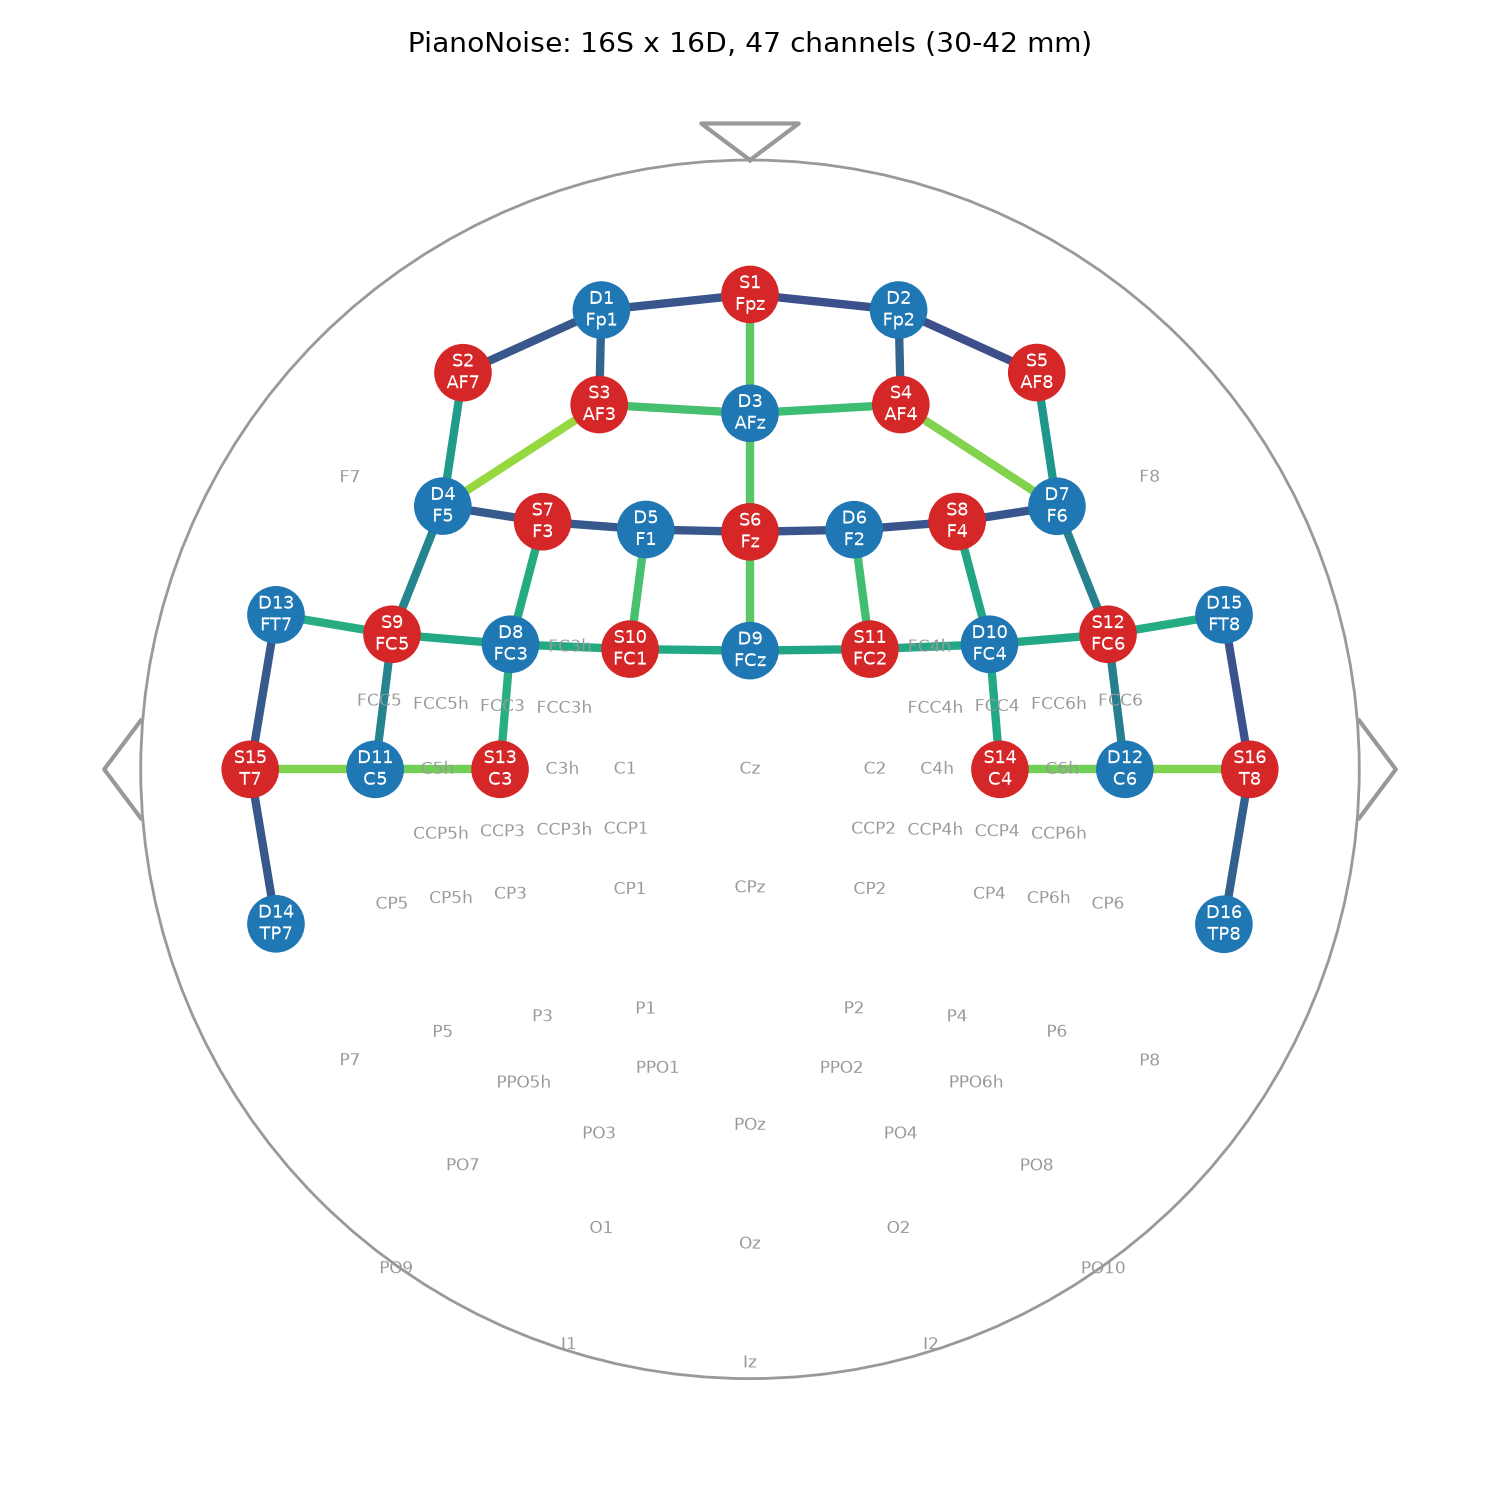
\includegraphics[width=0.62\textwidth]{figures/montage_2d.png}
\caption{The \texttt{PianoNoise} montage, top view (nose up). Red: sources S1--S16, blue: detectors D1--D16, lines: the 47 channels (colour = source--detector distance, 30--42\,mm). Unused 10-10 sites in grey.}
\label{fig:montage}
\end{figure}

\subsection{fNIRS preprocessing}
Preprocessing was performed in NIRWizard 0.1.7 using its cedalion backend (v26.5.2), starting from the \texttt{cedalion-recommended} pipeline with the modifications listed below; the as-executed parameters are stored in the analysis sidecars. The four recordings (quiet\_1, noise\_1, quiet\_2, noise\_2) were treated as four runs of one session. Raw intensities at 760 and 850\,nm were converted to optical density relative to the temporal mean of each channel. Motion artefacts were corrected in three steps: PCA-based artefact removal on segments detected by amplitude/standard-deviation thresholds (\texttt{tMotion}=0.5\,s, \texttt{tMask}=1\,s, STDEV 50, AMP 5; 97\,\% of variance, 15 components, 9 segments of 2--5\,s), followed by temporal derivative distribution repair (TDDR) and wavelet-based correction (db2, 4 levels, IQR 1.5). The corrected OD signals were band-pass filtered between 0.01 and 0.5\,Hz (4th-order zero-phase Butterworth, effective order 8) to remove slow drift and cardiac pulsation. Concentration changes of HbO and HbR ($\mu$M) were computed with the modified Beer--Lambert law using Prahl extinction coefficients, the measured source--detector distances and age-dependent differential pathlength factors (Scholkmann \& Wolf 2013; age 25 assumed; DPF 6.15 / 5.09 at 760 / 850\,nm). The data were finally resampled from 12.2 to 10\,Hz (anti-aliased), giving 21\,429 samples (2\,143\,s). Channel quality was assessed with windowed scalp-coupling index and peak spectral power, but no channel was excluded from the analysis reported here (Section~\ref{sec:qc}); no short-separation regression was possible because the montage has no short channels.

\subsection{GLM}
Subject-level GLM with one boxcar regressor per condition (QUIET, NOISE; event duration 40\,s) convolved with the canonical SPM HRF (kernel 32\,s, peak delay 6\,s, undershoot delay 16\,s, ratio 6, no derivatives), per-run DCT drift terms (cutoff 128\,s, 31 columns), three run-intercept columns and a global intercept. The solver was AR-IRLS (Barker, Aarabi \& Huppert 2013): Yule--Walker AR prewhitening with BIC order selection up to 40 samples (4\,s; selected orders 8--33), pooled over runs and restarted at every run seam, with Tukey-bisquare robust weights. Inference is per channel on the canonical-HRF $\beta$ with $\mathrm{dfe}=n-p=21\,392$ and Benjamini--Hochberg FDR within each condition $\times$ chromophore family. No QUIET-vs-NOISE contrast was fitted; the two conditions are compared descriptively. NIRWizard flags that the 0.01\,Hz high-pass and the 128\,s DCT cutoff overlap (both filters are in the record).

Cortical renders were exported from NIRWizard (GLM $t$, HbO, cortex opaque, probe hidden, 800$\times$800) in two versions: unthresholded, and with a descriptive display threshold $|t|>10$. With $\mathrm{dfe}\approx 21\,000$ the $t$ values are large everywhere; the $|t|>10$ cut is not a significance level but a way of showing only the strongest channels.

\section{Results}

\subsection{Play-related activation in both conditions}
Playing increased HbO almost everywhere the montage looks: 45/47 channels in QUIET and 44/47 in NOISE survive $q<0.05$, with positive $\beta$ in all but a few channels (up to 0.41\,$\mu$M). HbR is far weaker (27 and 30 channels at $q<0.05$, mixed sign, $|\beta|\le0.1\,\mu$M) and the canonical HbO-up/HbR-down pattern is present in only part of the montage; laterality is therefore reported for HbO. Figure~\ref{fig:unthr} shows the unthresholded HbO $t$-maps. In both conditions the strongest channels are the frontal-pole row (Fpz--Fp1/Fp2/AFz, $t=11$--13), left premotor/motor (FC5--C5, $t=13.5$ and $11.5$) and left temporal (T7--C5, $t=10.7$). Both maps look bilateral at this level; the difference between them is one of degree in the right lateral channels.

\begin{figure}[htbp]
\centering
\setlength{\tabcolsep}{1pt}
\begin{tabular}{cccc}
\viewrow{no_threshold}{QUIET}\\
\viewrow{no_threshold}{NOISE}\\
\small Left & \small Right & \small Anterior & \small Superior
\end{tabular}
\caption{Unthresholded GLM $t$ (HbO) projected on the cortex. Top row: QUIET, bottom row: NOISE. Columns: left lateral, right lateral, anterior, superior view. Colour scale $\pm14$.}
\label{fig:unthr}
\end{figure}

\subsection{Thresholded maps: a right-hemisphere cluster appears only in noise}
At $|t|>10$ (Fig.~\ref{fig:thr}) exactly 13 HbO channels survive in each condition, but not the same 13 (Table~\ref{tab:t10}). In QUIET, 7 are left-hemisphere, 2 midline and 4 right, and the right ones are all prefrontal (Fpz--Fp2, AF4--AFz, FC2--FCz) plus FC6--FT8. In NOISE, 6 are left, 1 midline and 6 right, and three right channels enter that are far below threshold in QUIET: T8--FT8 ($t$ 5.0 $\rightarrow$ 12.6, $\beta$ 0.09 $\rightarrow$ 0.23\,$\mu$M), FC6--C6 (5.9 $\rightarrow$ 12.5, 0.15 $\rightarrow$ 0.32\,$\mu$M) and T8--C6 (7.2 $\rightarrow$ 11.0, 0.13 $\rightarrow$ 0.20\,$\mu$M). Together with FC6--FT8 (above threshold in both) they form a contiguous right temporal--ventral premotor strip, visible as the large red patch in the right lateral NOISE view and as the right-lateral extension in the superior view. The neighbouring right channels C4--C6 and AF8--F6 also rise (7.5 $\rightarrow$ 8.8 and 5.1 $\rightarrow$ 8.8) without reaching the cut. On the left, the mirror channels do not change or fall slightly (T7--FT7 8.5 $\rightarrow$ 5.9; FC5--FT7 10.3 $\rightarrow$ 5.7; T7--C5 10.7 $\rightarrow$ 10.7; FC5--C5 13.5 $\rightarrow$ 11.5). The left lateral view is therefore near-identical across conditions, whereas the right lateral view is not.

\begin{figure}[htbp]
\centering
\setlength{\tabcolsep}{1pt}
\begin{tabular}{cccc}
\viewrow{thershold_t10}{QUIET}\\
\viewrow{thershold_t10}{NOISE}\\
\small Left & \small Right & \small Anterior & \small Superior
\end{tabular}
\caption{The same maps thresholded at $|t|>10$ (descriptive). Top: QUIET, bottom: NOISE. The right temporal--premotor cluster (T8--FT8, FC6--C6, T8--C6, FC6--FT8) is present only in NOISE (right lateral and superior views); the left lateral view is essentially unchanged.}
\label{fig:thr}
\end{figure}

\begin{table}[htbp]
\centering\small
\caption{HbO channels with $t\ge10$ in either condition (subject GLM, $\mathrm{dfe}=21\,392$; all $q<10^{-6}$). $\beta$ in $\mu$M. Bold: channels that cross the $t=10$ cut in one condition only. Hemisphere as assigned by NIRWizard's laterality ROI (midline-anchored channels AF4--AFz and FC2--FCz count as right, AF3--AFz and FC1--FCz as left).}
\label{tab:t10}
\begin{tabular}{llc rr rr}
\toprule
& & & \multicolumn{2}{c}{QUIET} & \multicolumn{2}{c}{NOISE}\\
\cmidrule(lr){4-5}\cmidrule(lr){6-7}
Channel & Sites & Hemi. & $\beta$ & $t$ & $\beta$ & $t$\\
\midrule
S16--D15 & T8--FT8   & R & 0.090 & 5.01  & \textbf{0.226} & \textbf{12.55}\\
S12--D12 & FC6--C6   & R & 0.148 & 5.88  & \textbf{0.319} & \textbf{12.54}\\
S16--D12 & T8--C6    & R & 0.130 & 7.21  & \textbf{0.201} & \textbf{11.00}\\
S12--D15 & FC6--FT8  & R & 0.163 & 12.06 & 0.173 & 12.69\\
S1--D2   & Fpz--Fp2  & R & 0.350 & 10.72 & 0.391 & 11.94\\
S4--D3   & AF4--AFz  & R & 0.235 & 12.19 & 0.197 & 10.08\\
S11--D9  & FC2--FCz  & R & \textbf{0.148} & \textbf{10.75} & 0.082 & 5.93\\
\addlinespace
S1--D3   & Fpz--AFz  & M & 0.336 & 13.30 & 0.303 & 11.86\\
S6--D3   & Fz--AFz   & M & \textbf{0.188} & \textbf{10.87} & 0.154 & 8.82\\
\addlinespace
S9--D11  & FC5--C5   & L & 0.289 & 13.47 & 0.250 & 11.55\\
S1--D1   & Fpz--Fp1  & L & 0.350 & 11.84 & 0.379 & 12.75\\
S2--D1   & AF7--Fp1  & L & 0.410 & 11.28 & 0.395 & 10.80\\
S15--D11 & T7--C5    & L & 0.148 & 10.75 & 0.149 & 10.68\\
S7--D4   & F3--F5    & L & \textbf{0.182} & \textbf{12.12} & 0.103 & 6.79\\
S9--D13  & FC5--FT7  & L & \textbf{0.205} & \textbf{10.29} & 0.115 & 5.72\\
S10--D5  & FC1--F1   & L & \textbf{0.151} & \textbf{10.19} & 0.110 & 7.36\\
S7--D5   & F3--F1    & L & 0.053 & 6.77  & \textbf{0.084} & \textbf{10.66}\\
S13--D11 & C3--C5    & L & 0.204 & 9.85  & \textbf{0.221} & \textbf{10.50}\\
\bottomrule
\end{tabular}
\end{table}

\subsection{Laterality}
NIRWizard's Seghier index over the two hemispheres, computed from the HbO $t$ values, is $\mathrm{LI}=+0.121$ in QUIET ($L=8.10$, $R=6.35$) and $+0.057$ in NOISE ($L=7.52$, $R=6.70$): mildly left-dominant while playing in quiet, and close to symmetric in noise. The shift is driven by the right lateral channels above; the left-hemisphere mean falls slightly.

\subsection{Data quality}\label{sec:qc}
Windowed QC (SCI $\ge0.8$, PSP $\ge0.1$, 421 windows) flags 27 of 47 channels as \emph{bad} (good-window fraction below 0.75), mostly on the PSP criterion (25 channels; 12 also fail SCI; none fail SNR, 12--65\,dB). The flagged channels are concentrated in the DLPFC/premotor rows and include several of the channels in Table~\ref{tab:t10}: FC6--C6 (0\,\% good windows), FC6--FT8 (62\,\%), FC5--C5 (72\,\%), Fpz--Fp1 (67\,\%), Fpz--Fp2 (60\,\%). The temporal channels T8--FT8, T8--C6 and T7--C5 pass; T7--FT7 does not (0\,\%). These verdicts were \emph{not} applied to the GLM (\texttt{qc\_applied: false}); a re-run with pruning, or with the PSP threshold relaxed, is needed to see whether the FC6--C6 result survives. Nine short motion segments (2--5\,s) were annotated by the PCA step, seven of them in the two NOISE runs.

\section{Interpretation and caveats}
The clearest single-subject observation is that playing in pink noise recruits a right temporal/ventral-premotor region (T8--FT8, T8--C6, FC6--C6, i.e.\ roughly right superior/middle temporal gyrus and inferior precentral/frontal operculum) that is only weakly engaged in quiet, while the left premotor/motor and prefrontal play response is unchanged. This is consistent with the study's premise that background noise adds an auditory-monitoring load on top of the motor task. Two properties of the setup argue for caution before calling it a noise effect: the loudspeaker stood on the player's \emph{left}, so the added right-temporal signal is on the side contralateral to the noise source and could in part be a direct auditory response to the noise rather than to playing-in-noise; and no QUIET$>$NOISE / NOISE$>$QUIET contrast was fitted, so the difference between the two maps has not been tested. Further limitations: $n=1$ (12 blocks per condition); no short-separation channels or ECG, so systemic contributions cannot be regressed out; HbR shows no corresponding decrease in the right temporal channels ($t$ between $-0.2$ and $+3.3$), which weakens the case for a purely neuronal origin; and QC was not applied. The $|t|>10$ threshold is purely descriptive. For the cohort study the obvious next steps are a NOISE--QUIET contrast in the same model, QC-pruned re-analysis, counterbalanced speaker placement (or diffuse noise), and short-separation channels.

\section*{Data provenance}
All numbers are taken from the NIRWizard 0.1.7 exports in \texttt{piano-noise/report/}: \texttt{quiet\_vs\_noise\_glm\_results.json} and \texttt{\_glm\_channels.csv} (GLM), \texttt{laterality.json}/\texttt{.csv}, \texttt{qc\_channels.json}/\texttt{.tsv}, \texttt{block\_average.json} and the cortex renders under \texttt{no\_threshold/} and \texttt{thershold\_t10/}. Sources: \texttt{data/dur40/\{quiet\_1,quiet\_2,noise\_1,noise\_2\}.snirf} (SHA-256 recorded in each sidecar). Session and montage details from \texttt{piano-noise/README.md}, \texttt{data/sessions.csv} and \texttt{data/blocks.csv}.

\end{document}
